\documentclass[a4paper,man,natbib]{apa6}

\usepackage[english]{babel}
\usepackage[utf8x]{inputenc}
\usepackage{amsmath}
\usepackage{graphicx}
\usepackage[colorinlistoftodos]{todonotes}
\usepackage{xcolor}
\usepackage[draft,inline,nomargin,index]{fixme}
\usepackage{hyperref}

\fxsetup{theme=color,mode=multiuser}
\FXRegisterAuthor{ab}{sab}{\color{blue}Amelie} % abnote{} with text inside to edit
\FXRegisterAuthor{bb}{sbb}{\color{purple}Brice} % bbnote{} with text inside to edit
\FXRegisterAuthor{ln}{sln}{\color{violet}Lad} % lnnote{} with text inside to edit

\title{Possible biasedness of the sequential testing procedure}
%\title{Preventing a possible bias of the sequential testing procedure}
%\title{Blinding as a remedy for demand biases during sequential testing}
\shorttitle{Blind Bayes Factor}
\threeauthors{Amélie G. Bret}{Brice Beffara}{Ladislas Nalborczyk}
\threeaffiliations{Univ. Grenoble Alpes, CNRS, LPNC UMR 5105, F-38000, Grenoble \\Psychological Science Research Institute, Catholic University of Louvain, Belgium}{The Walden III Slowpen Science Laboratory, France}{Univ. Grenoble Alpes, CNRS, LPNC UMR 5105, F-38000, Grenoble \\ Department of Experimental Clinical and Health Psychology, Ghent University}

\abstract{When collecting data, bayesian hypothesis testing allows optional stopping with unlimited multiple testing. This procedure is called Sequential Bayes Factors (SBF). Bayes factors are
computed until an a priori defined level of evidence is reached. This allows flexible sampling plans and
is not dependent upon correct effect size guesses in an a priori power analysis. Testing mean differences between 2 groups, the SBF design typically needs 50\% to 70\% smaller samples to reach a conclusion
about the presence of an effect,  as compared
with optimal NHST, while having the same or lower long-term rate of wrong inference. \todo[inline, color=red]{Le début de l'asbtract est extrait de pain joli et al. Il faudra le reformuler.}}

\begin{document}
\maketitle

\section{Introduction}

\lnnote{Où publier ? S'il s'agit d'un commentaire, il doit être publié dans la même revue que l'article original. Il y a deux papiers qui présentent la méthode SBF, un dans Psych. Meth (2017) et l'autre dans PBR (in press). \newline PBR accepte les commentaires : "Commentaries on previously published articles also appear in the journal...": http://www.springer.com/psychology/cognitive+psychology/journal/13423/PS2?detailsPage=aboutThis \newline Je ne sais pas si Psych. Meth les accepte...}

\bbnote{Exact mais Psych Meth accepte aussi des tuto donc on pourrait peut-être faire passer ça comme un tuto non ?}

\lnnote{Ça me semble un peu léger pour un tuto... non ? On présenterait quoi ? juste une fonction qui ajoute un argument "blind" aux fonctions existantes ? Ça ferait un bon article de blog mais je pense que c'est un peu léger pour un tuto...PS: je pense que Psych. Meth. accepte les comments, même s'ils ne le précisent, mais il faudrait juste s'en assurer... je peux m'occupper de vérifier ça}

\section{Proposition de plan}

\renewcommand{\labelenumii}{\Roman{enumii}}
\begin{enumerate}
	\item{Introduction, état du problème}
	\begin{enumerate}
		\item{Présentation de la méthode SBF}
		\item{Problèmes}
			\begin{enumerate}
            \item{Non-respect de l'hypothèse d'indépendance des observations}
            \item{Biais de demande...}
            \end{enumerate}
            \end{enumerate}
            \item{Solutions, comment régler le problème ?}
            \begin{enumerate}
            \item{Blinding: soit triple blind (expé != analyst), soit blinding via software, cf. point suivant}
            \item{On peut proposer ici une solution pratique immédiate, genre une version modifiée de la fonction de félix qui ajouter un argument "blind" (en cours...)}
            \end{enumerate}
            \item{Evaluation du biais ?}
            \begin{enumerate}
            \item{Propositions de protocoles expérimentaux permettant de mettre en évidence le biais, prédictions.}
            \item{On pourrait profiter de ce papier pour lancer un appel à contribution à une grosse manip multi-lab all around the world, pour évaluer l'amplitude de ce biais, comme on avait commencé à discuter...non ?}

\end{enumerate}
\end{enumerate}

\bbnote{super idée j'aime cet séquence évolutive vmvc}

\section{Sondage et liste des arguments pour ou contre inclure Wagenmakers, Schönbrodt, Perugini et cie ?}

\textbf{Pour}: ils sont forts, ils peuvent nous éviter de dire des bêtises, ça fait moins "attaque" s'ils sont aussi auteurs...

\textbf{Contre}: on peut les avoir en reviewers... et ça fait une diversité de point de vues dans la littérature (genre moins crew)

\section{TO-DO}

\begin{itemize}

\item{trouver un acronyme sexy pour décrire le biais, genre le "Sequential Experimenter-as-Analyst Bias" (SEAB).}

\item{revue de littérature sur le biais de l'expérimentateur, travaux récents ? estimation de la taille d'effet ?}

\item{insérer un diagramme qui représente le processus de sequential testing et là où opère notre biais potentiel...}

\item{insérer un diagramme de nos prédictions...}

\item{modifier la fonction seqBF de Richard Morey et Félix Schonbrodt afin d'ajouter un argument "blind"} \lnnote{DONE}

\end{itemize}

\section{misc}

(private) repo github: \url{https://github.com/lnalborczyk/Blind_BF}

test citation...\cite{kruschke_bayesian_2017}...

\section{Supplementary materials}

...

\section{Acknowledgements}

...

% Commands to include a figure:
%\begin{figure}
%\centering
%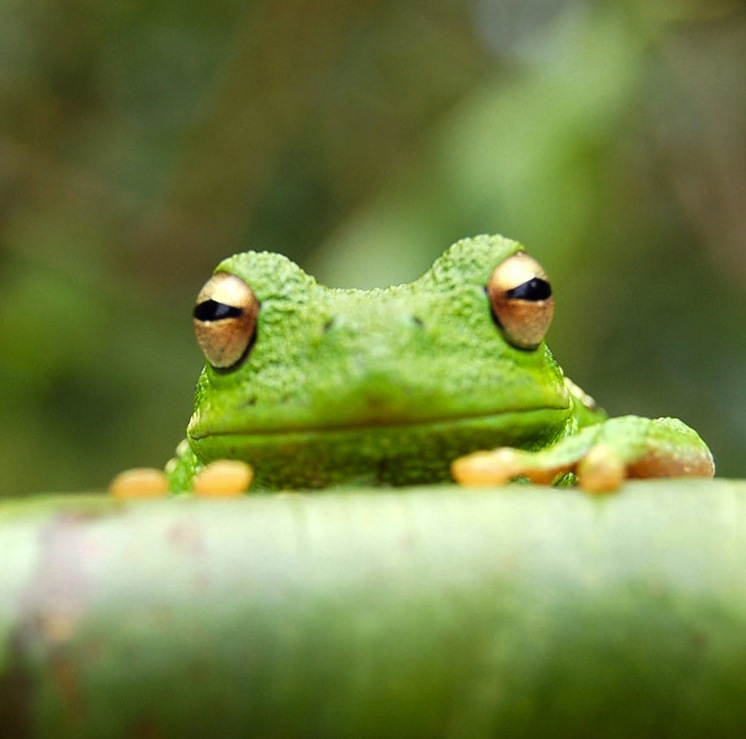
\includegraphics[width=0.5\textwidth]{frog.jpg}
%\caption{\label{fig:frog}This is a figure caption.}
%\end{figure}

\bibliography{Zotero}
\end{document}
